\chapter{Lecture 27 - Embedded RK and MATLAB Built-in RK Methods}
\label{ch:lec27n}
\section{Objectives}
The objectives of this lecture are to:
\begin{itemize}
\item Describe an demonstrate embedded Runge-Kutta methods as they relate to adaptive step-sizing
\item Introduce MATLAB Built-in RK Methods
\item Illustrate their use through example problems.
\end{itemize}
\setcounter{lstannotation}{0}

\section{Embedded Runge-Kutta Methods}
Besides developing methods to achieve higher order accuracy, there is also an incentive to minimize the required number of time steps while also achieving a specified absolute or relative error.  In the preceding examples, the user has been called upon to input the desired time step size and interval over which the calculation is to be made and it was left for the user to decide if the time step size is appropriate.  But if we consider the problem from a somewhat higher level, we would not expect the user to be focused on the time step size but rather whether or not the solution is accurate enough.  The user should input the expected relative or absolute error tolerance instead of details about how many time steps to make or how big those steps should be.

What we need are:
\begin{enumerate}
\item A way to estimate the error in a solution; and
\item the means of making this estimate should not require a lot more work.
\end{enumerate}  

Embedded Runge-Kutta methods provide for those needs.  Consider the Bogacki-Shampine method that is used in MATLAB's built-in function \lstinline[style=myMatlab]{ode23}.\cite{bogacki19893} The Butcher tableau is shown in Table \ref{tab:lec27n-bs-bt}.


\begin{margintable}[-8.0cm]
\begin{tabular}{c|cccc}
0 & 0 & 0 & 0 & 0 \\
\sfrac{1}{2} & \sfrac{1}{2} & 0 & 0 & 0 \\
\sfrac{3}{4} & 0 & \sfrac{3}{4} & 0 & 0 \\
1 & \sfrac{2}{9} & \sfrac{1}{3} & \sfrac{4}{9} & 0 \\ \hline
(2) & \sfrac{7}{24} & \sfrac{1}{4} & \sfrac{1}{3} & \sfrac{1}{8} \\
(3) & \sfrac{2}{9} & \sfrac{1}{3} & \sfrac{4}{9} & 0
\end{tabular}
\caption{Butcher tableau for the Bogacki-Shampine embedded Runge-Kutta method.}
\label{tab:lec27n-bs-bt}
\end{margintable}
In this Butcher tableau, there are two sets of weights: one for a 2\textsuperscript{nd}-order convergent RK method and the other is for a 3\textsuperscript{rd}-order convergent scheme. Note that the numbers to the left of the weights in the Butcher tableau are not standard and added to indicate the order of convergence for the corresponding set of weights.

This can form the basis for a step-size adaptation method.  Suppose we specify a relative error tolerance and compute $y_{n+1}$ given $y_n$.  
\begin{itemize}
\item Start with a default initial step size.  This might be input by the user or may be set by the algorithm, for example, as a fixed fraction of the interval length. 
\item Compute the numeric solution for the $(i+1)$-th time-step using both lower-order and higher-order weights ($w_{i+1}$ and $z_{i+1}$, respectively)
\item Obtain a measure of the relative error from the two solutions.\marginnote{\textbf{Note:} Since the system is, in general, n\textsuperscript{th}-order, $w$ and $z$ are generally vectors of length $n$. Choose a suitable norm in which to obtain this relative error measure. In order to guard against small values of $||z_{i+1}||$, use a tool like \lstinline[style=myMatlab]{min(z,theta)}, where \lstinline[style=myMatlab]{theta} is a small non-zero value. }
\begin{equation*}
e_{i+1} \approx \frac{||w_{i+1}-z_{i+1}||}{||z_{i+1}||}
\end{equation*}
\item If the relative error measure fails to meet the specified error tolerance, we reduce the step size---for instance, $h_{new} = \sfrac{h}{2}$---and re-compute.
\item If the relative error tolerance is satisfied, we specify a larger step size for the next time step. One equation for doing this is shown in Equation \ref{eq:lec27n-step-size-change} where $p$ is the order of the solver, $h$ is the time step size, $e_{i+1}$ is the error measure, and SF is a chosen \emph{safety factor} that, by setting to a value between 0 and 1, prevents changing the time step size too aggressively.\cite{sauer2011numerical}

\begin{equation}
h_{\text{new}}=(SF)\left(\frac{\text{TOL}}{e_{i+1}}\right)^{\frac{1}{p+1}}h_{\text{old}}
\label{eq:lec27n-step-size-change}
\end{equation}

\item Ensure the final time-step is sized so that the algorithm terminates at the end of the specified interval.

\end{itemize}

One possible implementation of this method is shown in the set of listings below.
\marginnote{

\vspace{0.4cm}

\noindent\ref{lst:ann27n-1} The last argument, \lstinline[style=myMatlab]{EBT}, is what we will call the \emph{extended} Butcher tableau, so-called because it is extended to contain two sets of weights.

\vspace{0.25cm}

\noindent\ref{lst:ann27n-2} For this method we do not know in advance how many timesteps will be taken but we also want to pre-allocate arrays for our variables.  Consequently we will make a conservative guess at the number of timesteps necessary.  At the end of the array we will trim away unused portions of the array.
}
\begin{lstlisting}[style=myMatlab, name=lec27n-1]
function [t,y] = embeddedRK(F,tspan,y0,RTOL,EBT) /*!\annotation{lst:ann27n-1}!*/
t_sz = 5000; % initial size for output arrays
tsMax = 100000;
sys_size = length(y0);
t = nan(1,t_sz); /*!\annotation{lst:ann27n-2}!*/
y = nan(sys_size,t_sz);
\end{lstlisting}

\noindent Now we unpack the Butcher tableau and initialize our variables.

\begin{lstlisting}[style=myMatlab,name=lec27n-1]
% set initial values
t(1) = tspan(1);
y(:,1) = y0;

[m,~] = size(EBT);
s = m-2;
C = EBT(1:s,1); /*!\annotation{lst:ann27n-3}!*/
A = EBT(1:(end-2),2:end);
BW = EBT(s+1,2:end);
BZ = EBT(s+2,2:end);
p = EBT((end-1),1);
\end{lstlisting}
\marginnote[-2.0cm]{

\noindent\ref{lst:ann27n-3} Here we unpack the Butcher tableau with the only difference being that we have two sets of weights to use in the low order $w$ and high order $z$ approximation.
}
\noindent The rest of the implementation follows; the local function \lstinline{style=myMatlab}{getWZ()} will be shown in the next listing.

\marginnote{

\vspace{0.35cm}

\noindent\ref{lst:ann27n-4} This is the small factor to ensure the normalization used in calculating relative error is not too close to zero.

\vspace{2.5cm}

\noindent\ref{lst:ann27n-5} With each time step we need to find the right step-length.  We will use an iterative process starting with the time step size from the previous time step.

\vspace{3.0cm}

\noindent\ref{lst:ann27n-6} Move this process out to a different local function.

\vspace{0.10cm}

\noindent\ref{lst:ann27n-7} Use the two sets of weights to get the low-order ($w$) and high-order ($z$) approximation.

\vspace{0.5cm}

\noindent\ref{lst:ann27n-8} If the max relative error is within the relative error tolerance, accept the solution but also update the time step size for the next time around.

\vspace{0.5cm}

\noindent\ref{lst:ann27n-9} If the relative error tolerance is not met, cut the time stepsize in half and try again.

\vspace{0.5cm}

\noindent\ref{lst:ann27n-10} If it takes more than a couple of iterations, something has went wrong; stop the program and try to figure it out.
}
\begin{lstlisting}[style=myMatlab,name=lec27n-1]
SF = 0.9; % "safety factor"
theta = 1e-14; /*!\annotation{lst:ann27n-4}!*/
tStart = tspan(1);
tEnd = tspan(2);
h = (tEnd-tStart)/10; % initial step size
h_new = h;
stopFlag = 0; % flag to end on last time step

for ts = 1:tsMax
    cT = t(ts); % current time
    
    % find acceptable time step size  /*!\annotation{lst:ann27n-5}!*/
    int_it_count = 0; % limit iterations in error control.
    while int_it_cout < 10
        int_it_count = int_it_count + 1;
        h = h_new; % update with new step-size
        
        % if cT + h > tEnd, reduce h so we stop right on time
        if cT+h > tEnd 
           h = tEnd-cT; 
           stopFlag = 1; % stop after this time step
        end
        
        y(:,ts+1) = y(:,ts);
        K = getSlopeEst(F,t(ts),y(:,ts),h,C,A); /*!\annotation{lst:ann27n-6}!*/
        [w,z] = getWZ(y(:,ts),h,K,BW,BZ); /*!\annotation{lst:ann27n-7}!*/
        err_ts = abs(w-z); % error vector (length = # dofs)
        rel_err_ts = err_ts./max(abs(z),theta);
        max_rel_err_ts = norm(rel_err_ts,inf);
        if max_rel_err_ts < RTOL  /*!\annotation{lst:ann27n-8}!*/
            h_new = SF*(RTOL/max_rel_err_ts)^(1/(p+1))*h;  
            y(:,ts+1) = z; 
            t(ts+1) = cT + h; % update current time   
            break; % exit the while loop
        else
            h_new = h/2; /*!\annotation{lst:ann27n-9}!*/
            if stopFlag == 1
                stopFlag = 0;
            end
        end % if max_rel_err_ts...

        if int_it_count > 10 /*!\annotation{lst:ann27n-10}!*/
            error('Error-control is broken!'); 
        end
\end{lstlisting}
\setcounter{lstannotation}{0}
\begin{lstlisting}[style=myMatlab,name=lec27n-1]      
    end % while 
        
    if stopFlag == 1 % end of time stepping.  exit loop.
        break;
    end
end %ts
% trim the output variables.
y = y(:,1:(ts+1));  /*!\annotation{lst:ann27n-11}!*/
t = t(1:(ts+1));
end % function
\end{lstlisting}
\marginnote[-1.5cm]{
\noindent\ref{lst:ann27n-11} Recall, the variable arrays were over-sized to accomodate an unknown number of time steps.  Trim-off any unused time steps here.

}
The local functions used above are shown here for completeness.
\begin{lstlisting}[style=myMatlab,name=lec27n-1]
function K = getSlopeEst(F,t,y,h,C,A)
sys_size=length(y);% gen # of dep vars
[s,~] = size(A); % get number of stages
K = zeros(sys_size,s);
K(:,1) = F(t,y);
for i = 2:s
    y_it = y(:);
    x_it = t + C(i)*h;
    for j = 1:(i-1)
        y_it = y_it + h*A(i,j)*K(:,j);
    end %j    
    K(:,i) = F(x_it,y_it);
end %i
end

function [w,z] = getWZ(y,h,K,BW,BZ)
s = length(BW);
w = y; z = y;
for i = 1:s
   w = w + h*BW(i)*K(:,i);
   z = z + h*BZ(i)*K(:,i);
end
end
\end{lstlisting}
We use this embedded Runge-Kutta method to solve example \#2 from Lecture 25:

\begin{equation*}
4y^{\prime \prime}+4y^{\prime} + 17y=0, \ \ y(0)=-1, \ y^{\prime}(0)=2
\end{equation*}
with exact solution:
\begin{equation*}
y(x)=e^{-\sfrac{x}{2}}\left[-\cos{(2x)}+\frac{3}{4}\sin{(2x)} \right]
\end{equation*}
\begin{marginfigure}
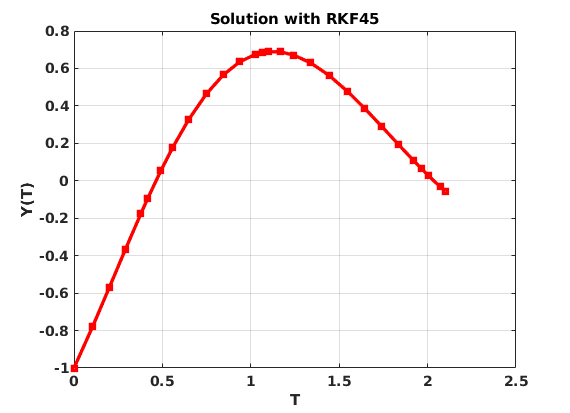
\includegraphics{lec27n-ex1.png}
\caption{Solution of example problem with an embedded Runge-Kutta method.}
\label{fig:lec27n-ex1}
\end{marginfigure}
A plot of the solution is shown in Figure \ref{fig:lec27n-ex1}.  Note the shorter timesteps in the vicinity of rapid solution variation or inflection points.

\section{MATLAB Built-in Runge-Kutta Methods}

MATLAB has a number of built-in methods for solving initial value problems.  
